
\section*{Kapitel 1 - Das einfache lineare Regressionsmodell}

\begin{multicols*}{3}

\tikzstyle{mybox} = [draw=black, fill=white, very thick,
    rectangle, rounded corners, inner sep=10pt, inner ysep=10pt]
\tikzstyle{fancytitle} =[fill=black, text=white, font=\bfseries]



%------------ Einfaches lineares Regressionsmodell ---------------
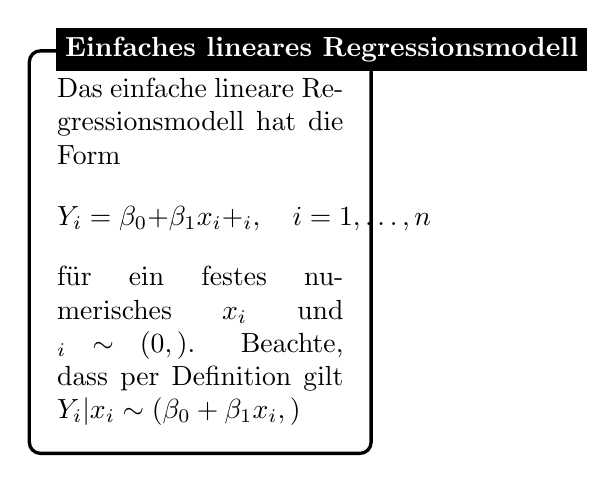
\begin{tikzpicture}
\node [mybox] (box){%
    \begin{minipage}{0.3\textwidth}
    Das \tc{einfache lineare Regressionsmodell} hat die Form $$Y_i = \beta_0 + \beta_1 x_i + \eps_i,\quad i = 1, \dots, n$$
    für ein festes numerisches $x_i$ und $\eps_i \sim \Ncal(0,\ssd)$.
    Beachte, dass per Definition gilt $Y_i| x_i \sim \Ncal(\beta_0 + \beta_1 x_i, \ssd)$
    \end{minipage}
};
%------------ Einfaches lineares Regressionsmodell Header ---------------------
\node[fill = black, text=white, font=\bfseries, right=10pt] at (box.north west) {Einfaches lineares Regressionsmodell};
\end{tikzpicture}

%------------ KQ Schätzer ---------------
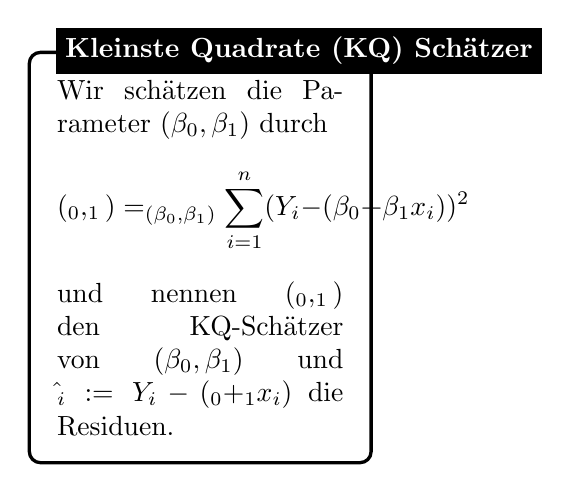
\begin{tikzpicture}
\node [mybox] (box){%
    \begin{minipage}{0.3\textwidth}
    Wir schätzen die Parameter $(\beta_0, \beta_1)$ durch 
    $$(\hbe_0, \hbe_1) = \argmin_{(\beta_0, \beta_1)} \sum_{i = 1}^n(Y_i - (\beta_0 + \beta_1 x_i))^2$$ und nennen $(\hbe_0, \hbe_1)$ den \tc{KQ-Schätzer von $(\beta_0, \beta_1)$} und $\hat{\eps}_i := Y_i - (\hbe_0 + \hbe_1 x_i)$ die \tc{Residuen}.
    \end{minipage}
};
%------------ KQ Schätzer Header ---------------------
\node[fill = black, text=white, font=\bfseries, right=10pt] at (box.north west) {Kleinste Quadrate (KQ) Schätzer};
\end{tikzpicture}

%------------ Existenz und Berechnung vom KQ Schätzer ---------------
\begin{tikzpicture}
\node [mybox] (box){%
    \begin{minipage}{0.3\textwidth}
    Der KQ-Schätzer existiert und ist eindeutig, falls $\sum_{i = 1}^n (x_i - \bar{x})^2 \neq 0$. Dieser lässt sich berechnen als 
    \begin{align*}
        \hbe_1 = & \quad \frac{s_{xY}}{S_x^2} = \frac{\frac1n\sum_{i = 1}^n (x_i - \bar{x})(Y_i - \bar{Y})}{\frac1n\sum_{i = 1}^n (x_i - \bar{x})^2}\\
        \hbe_0 = & \quad \bar{Y} - \hbe_1 \bar{x}
    \end{align*}
    \end{minipage}
};
%------------ Existenz und Berechnung vom KQ Schätzer Header --------
\node[fill = purple, text=white, font=\bfseries, right=10pt] at (box.north west) {Existenz und Berechnung vom KQ Schätzer};
\end{tikzpicture}













%------------ Überschrift ---------------

\begin{tikzpicture}
\node [mybox] (box){%
    \begin{minipage}{0.3\textwidth}
    
    \end{minipage}
};
%------------ Überschrift Header ---------------------
\node[fill = black, text=white, font=\bfseries, right=10pt] at (box.north west) {Überschrift};
\end{tikzpicture}

\end{multicols*}



